% Options for packages loaded elsewhere
% Options for packages loaded elsewhere
\PassOptionsToPackage{unicode}{hyperref}
\PassOptionsToPackage{hyphens}{url}
%
\documentclass[
  ignorenonframetext,
  aspectratio=169,
]{beamer}
\newif\ifbibliography
\usepackage{pgfpages}
\setbeamertemplate{caption}[numbered]
\setbeamertemplate{caption label separator}{: }
\setbeamercolor{caption name}{fg=normal text.fg}
\beamertemplatenavigationsymbolsempty
% remove section numbering
\setbeamertemplate{part page}{
  \centering
  \begin{beamercolorbox}[sep=16pt,center]{part title}
    \usebeamerfont{part title}\insertpart\par
  \end{beamercolorbox}
}
\setbeamertemplate{section page}{
  \centering
  \begin{beamercolorbox}[sep=12pt,center]{section title}
    \usebeamerfont{section title}\insertsection\par
  \end{beamercolorbox}
}
\setbeamertemplate{subsection page}{
  \centering
  \begin{beamercolorbox}[sep=8pt,center]{subsection title}
    \usebeamerfont{subsection title}\insertsubsection\par
  \end{beamercolorbox}
}
% Prevent slide breaks in the middle of a paragraph
\widowpenalties 1 10000
\raggedbottom
\usepackage{iftex}
\ifPDFTeX
  \usepackage[T1]{fontenc}
  \usepackage[utf8]{inputenc}
  \usepackage{textcomp} % provide euro and other symbols
\else % if luatex or xetex
  \usepackage{unicode-math} % this also loads fontspec
  \defaultfontfeatures{Scale=MatchLowercase}
  \defaultfontfeatures[\rmfamily]{Ligatures=TeX,Scale=1}
\fi
\usepackage{lmodern}

\usetheme[]{metropolis}
\ifPDFTeX\else
  % xetex/luatex font selection
\fi
% Use upquote if available, for straight quotes in verbatim environments
\IfFileExists{upquote.sty}{\usepackage{upquote}}{}
\IfFileExists{microtype.sty}{% use microtype if available
  \usepackage[]{microtype}
  \UseMicrotypeSet[protrusion]{basicmath} % disable protrusion for tt fonts
}{}
\makeatletter
\@ifundefined{KOMAClassName}{% if non-KOMA class
  \IfFileExists{parskip.sty}{%
    \usepackage{parskip}
  }{% else
    \setlength{\parindent}{0pt}
    \setlength{\parskip}{6pt plus 2pt minus 1pt}}
}{% if KOMA class
  \KOMAoptions{parskip=half}}
\makeatother


\usepackage{longtable,booktabs,array}
\usepackage{calc} % for calculating minipage widths
\usepackage{caption}
% Make caption package work with longtable
\makeatletter
\def\fnum@table{\tablename~\thetable}
\makeatother
\usepackage{graphicx}
\makeatletter
\newsavebox\pandoc@box
\newcommand*\pandocbounded[1]{% scales image to fit in text height/width
  \sbox\pandoc@box{#1}%
  \Gscale@div\@tempa{\textheight}{\dimexpr\ht\pandoc@box+\dp\pandoc@box\relax}%
  \Gscale@div\@tempb{\linewidth}{\wd\pandoc@box}%
  \ifdim\@tempb\p@<\@tempa\p@\let\@tempa\@tempb\fi% select the smaller of both
  \ifdim\@tempa\p@<\p@\scalebox{\@tempa}{\usebox\pandoc@box}%
  \else\usebox{\pandoc@box}%
  \fi%
}
% Set default figure placement to htbp
\def\fps@figure{htbp}
\makeatother





\setlength{\emergencystretch}{3em} % prevent overfull lines

\providecommand{\tightlist}{%
  \setlength{\itemsep}{0pt}\setlength{\parskip}{0pt}}



 


% ============================================================
%  Econ 2203 — Beamer Metropolis Theme Preamble
%  Course: International Trade and Policy in Agriculture
%  Instructor: Nithin M, Department of Development Economics
% ============================================================

% MUST be first: load Metropolis theme before \metroset and colour overrides
\usetheme{metropolis}

% Only load packages not already provided by pandoc's beamer template
\usepackage{amsmath,amssymb}

% ---- Brand colours -----------------------------------------
\definecolor{brandblue}{HTML}{012169}
\definecolor{brandgold}{HTML}{B9975B}
\definecolor{lightblue}{HTML}{E8EDF5}

% ---- Metropolis colour overrides ---------------------------
% Main palette
\setbeamercolor{normal text}{fg=black,bg=white}
\setbeamercolor{alerted text}{fg=brandgold}
\setbeamercolor{example text}{fg=brandblue!70!black}

% Title slide
\setbeamercolor{title}{fg=white,bg=brandblue}
\setbeamercolor{subtitle}{fg=brandgold}
\setbeamercolor{author}{fg=white}
\setbeamercolor{institute}{fg=brandgold!80!white}
\setbeamercolor{date}{fg=white}
\setbeamercolor{title page header}{fg=white,bg=brandblue}

% Frametitle bar
\setbeamercolor{frametitle}{fg=white,bg=brandblue}

% Progress bar → gold
\setbeamercolor{progress bar}{fg=brandgold,bg=brandblue!30}
\setbeamercolor{title separator}{fg=brandgold}
\setbeamercolor{progress bar in head/foot}{fg=brandgold,bg=brandblue!20}
\setbeamercolor{progress bar in section page}{fg=brandgold,bg=brandblue!20}

% Blocks
\setbeamercolor{block title}{bg=brandblue,fg=white}
\setbeamercolor{block body}{bg=lightblue,fg=black}
\setbeamercolor{block title alerted}{bg=brandgold,fg=white}
\setbeamercolor{block body alerted}{bg=brandgold!12,fg=black}
\setbeamercolor{block title example}{bg=brandblue!70!black,fg=white}
\setbeamercolor{block body example}{bg=brandblue!8,fg=black}

% Structure / lists
\setbeamercolor{structure}{fg=brandblue}
\setbeamercolor{section in toc}{fg=brandblue}
\setbeamercolor{itemize item}{fg=brandblue}
\setbeamercolor{itemize subitem}{fg=brandgold}
\setbeamercolor{enumerate item}{fg=brandblue}
\setbeamercolor{description item}{fg=brandblue}

% ---- Metropolis options ------------------------------------
\metroset{
  progressbar    = frametitle,   % gold bar under frametitle
  sectionpage    = none,
  numbering      = fraction,
  block          = fill
}

% ---- Fonts (Metropolis uses Fira Sans; fallback gracefully) -
\setbeamerfont{title}{size=\Large,series=\bfseries}
\setbeamerfont{subtitle}{size=\normalsize,series=\mdseries}
\setbeamerfont{frametitle}{size=\large,series=\bfseries}
\setbeamerfont{block title}{size=\normalsize,series=\bfseries}
\setbeamerfont{caption}{size=\footnotesize}

% ---- Footer: course info + slide number --------------------
\setbeamertemplate{footline}{%
  \begin{beamercolorbox}[wd=\paperwidth,ht=2.0ex,dp=1ex]{footline}%
    \hspace{0.8em}%
    {\footnotesize\color{brandblue!60}%
      Econ 2203 \textbar{} International Trade and Policy in Agriculture
      \hfill Nithin M \hfill
      \insertframenumber{}/\inserttotalframenumber\hspace{0.8em}}%
  \end{beamercolorbox}%
}

% ---- Misc --------------------------------------------------
\setlength{\parskip}{0.25em}
\setbeamertemplate{navigation symbols}{}

% tighter column sep for side-by-side content
\setlength{\columnsep}{0.8em}

% Fix: make \label truly robust in moving arguments (Quarto generates
% \caption{\label{fig-xxx}...} which crashes Metropolis in batchmode).
% DeclareRobustCommand creates a self-protecting robust version.
\makeatletter
\let\quarto@originallabel\label
\DeclareRobustCommand*{\label}[1]{\quarto@originallabel{#1}}
\makeatother

% Prevent figures from overflowing Beamer frames.
% width=\linewidth: scale to text width (already Quarto default);
% height=0.6\textheight: cap height so figures never push past the frame bottom.
% keepaspectratio: never distort — whichever constraint binds first wins.
\setkeys{Gin}{width=\linewidth,height=0.6\textheight,keepaspectratio}
\makeatletter
\@ifpackageloaded{caption}{}{\usepackage{caption}}
\AtBeginDocument{%
\ifdefined\contentsname
  \renewcommand*\contentsname{Table of contents}
\else
  \newcommand\contentsname{Table of contents}
\fi
\ifdefined\listfigurename
  \renewcommand*\listfigurename{List of Figures}
\else
  \newcommand\listfigurename{List of Figures}
\fi
\ifdefined\listtablename
  \renewcommand*\listtablename{List of Tables}
\else
  \newcommand\listtablename{List of Tables}
\fi
\ifdefined\figurename
  \renewcommand*\figurename{Figure}
\else
  \newcommand\figurename{Figure}
\fi
\ifdefined\tablename
  \renewcommand*\tablename{Table}
\else
  \newcommand\tablename{Table}
\fi
}
\@ifpackageloaded{float}{}{\usepackage{float}}
\floatstyle{ruled}
\@ifundefined{c@chapter}{\newfloat{codelisting}{h}{lop}}{\newfloat{codelisting}{h}{lop}[chapter]}
\floatname{codelisting}{Listing}
\newcommand*\listoflistings{\listof{codelisting}{List of Listings}}
\makeatother
\makeatletter
\makeatother
\makeatletter
\@ifpackageloaded{caption}{}{\usepackage{caption}}
\@ifpackageloaded{subcaption}{}{\usepackage{subcaption}}
\makeatother

\usepackage{bookmark}
\IfFileExists{xurl.sty}{\usepackage{xurl}}{} % add URL line breaks if available
\urlstyle{same}
\hypersetup{
  pdftitle={Lecture 18: India's Agricultural Trade and Foreign Trade Policy},
  pdfauthor={Nithin M},
  hidelinks,
  pdfcreator={LaTeX via pandoc}}


\title{Lecture 18: India's Agricultural Trade and Foreign Trade Policy}
\subtitle{Econ 2203 \textbar{} International Trade and Policy in
Agriculture}
\author{Nithin M}
\date{2026-08-22}
\institute{Department of Development Economics}

\begin{document}
\frame{\titlepage}


\begin{frame}{}
\phantomsection\label{section}
\textbf{Lecture 18 --- Final Lecture}

{India's Agricultural Trade and Foreign Trade Policy}

\emph{Bringing It All Together}
\end{frame}

\begin{frame}
\begin{block}{Opening Reflection}
\phantomsection\label{opening-reflection}
\begin{columns}[T]
\begin{column}{0.58\linewidth}
\textbf{Eighteen weeks ago, we asked:}

\begin{quote}
\emph{Why do countries trade? And what does that mean for the 600
million Indians who depend on agriculture for their livelihoods?}
\end{quote}

Today, we can answer that question \textbf{fully} --- with theory, data,
institutions, and policy.

We have traced the journey from Ricardo's simple insight about
comparative advantage, through the architecture of WTO rules, the
mechanics of import tariffs, the politics of MSP and food security, the
diplomacy of phytosanitary protocols, and the paperwork of a Shipping
Bill on ICEGATE.

\textbf{This is what Econ 2203 has been about.}
\end{column}

\begin{column}{0.42\linewidth}
\textbf{What we built, week by week:}

\begin{itemize}
\tightlist
\item
  \textbf{Weeks 1--2:} Why trade? Gains and features
\item
  \textbf{Weeks 3--6:} Theory --- Ricardo to Heckscher-Ohlin to New
  Trade Theory
\item
  \textbf{Weeks 7--8:} Protectionism --- tariffs, quotas, subsidies
\item
  \textbf{Weeks 9--10:} Balance of Payments and India's external sector
\item
  \textbf{Weeks 11--12:} Foreign exchange markets
\item
  \textbf{Weeks 13--14:} WTO, AoA, and India's negotiating positions
\item
  \textbf{Week 15:} SPS barriers --- India's compliance challenge
\item
  \textbf{Weeks 16--17:} Export procedures and organizations
\item
  \textbf{Week 18:} Today --- synthesis, FTP, and vision 2030
\end{itemize}
\end{column}
\end{columns}
\end{block}
\end{frame}

\begin{frame}
\begin{block}{The Full Chain: Course Synthesis Diagram}
\phantomsection\label{the-full-chain-course-synthesis-diagram}
\textbf{Course Synthesis: International Trade Logic Chain}

\begin{enumerate}
\tightlist
\item
  \textbf{Comparative Advantage} → countries gain from specialisation
\item
  \textbf{Gains from Trade} → mediated by terms of trade
\item
  \textbf{Trade Policy} → tariffs, quotas, subsidies shape distribution
\item
  \textbf{BOP \& Exchange Rates} → macro context for trade flows
\item
  \textbf{International Institutions} → WTO, AoA, SPS discipline policy
\item
  \textbf{India's Strategy} → Export promotion + selective protection
\end{enumerate}

\textbf{Every lecture has been one step in this chain.}

The central tension of the entire course:

{Free trade maximises efficiency} --- comparative advantage theory,
consumer gains, global welfare.

{But agriculture is not like other sectors} --- food is existential,
farming communities are politically powerful, and market failures
(information asymmetry, price volatility, public goods in R\&D) are
pervasive.

The discipline of agricultural trade economics is, fundamentally, the
study of how societies navigate this tension.
\end{block}
\end{frame}

\begin{frame}
\begin{block}{India's Foreign Trade Policy: Key Milestones}
\phantomsection\label{indias-foreign-trade-policy-key-milestones}
\begin{figure}

\centering{

\pandocbounded{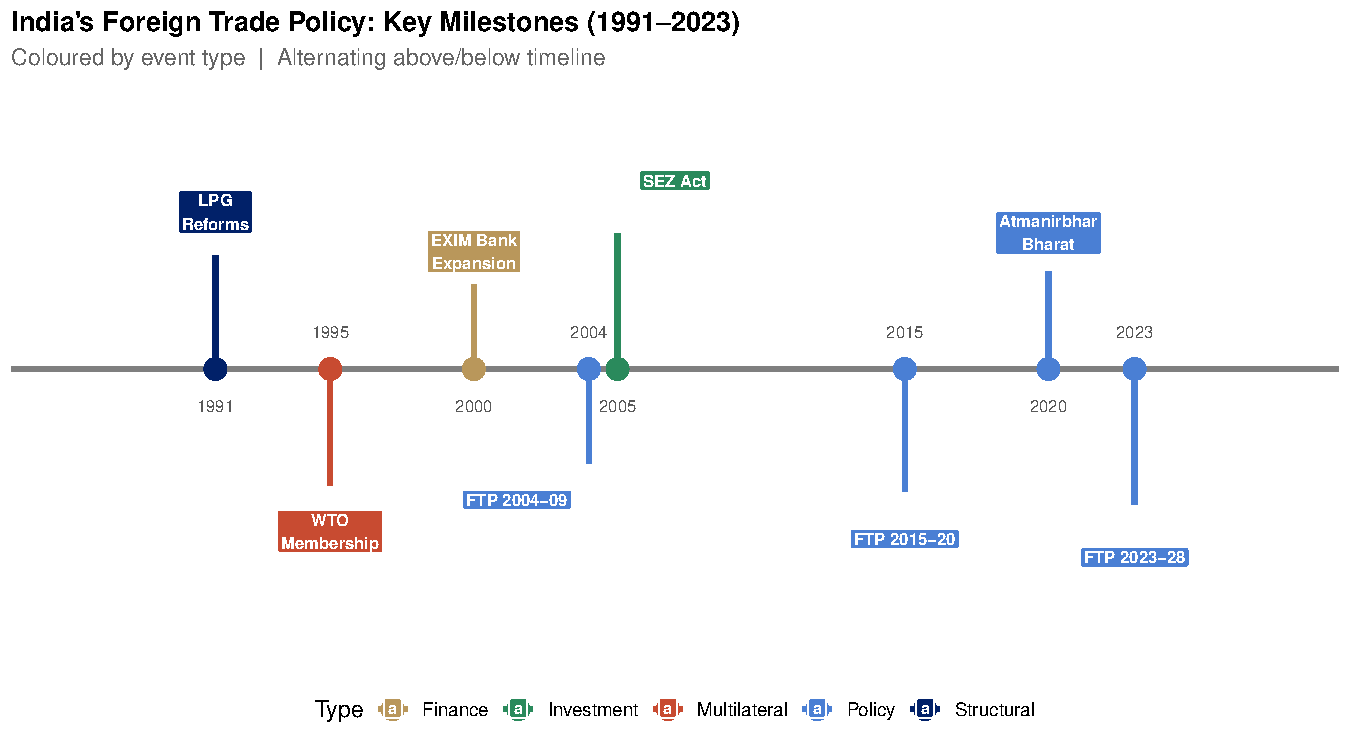
\includegraphics[keepaspectratio]{Lecture18_India_Agri_Trade_Policy_files/figure-beamer/fig-ftp-timeline-1.pdf}}

}

\caption{\label{fig-ftp-timeline}India's trade policy evolved from the
1991 LPG reforms through WTO accession and successive FTPs, culminating
in the landmark FTP 2023-28 targeting USD 2 trillion by 2030. Source:
DGFT, Ministry of Commerce and Industry, GoI.}

\end{figure}%
\end{block}
\end{frame}

\begin{frame}
\begin{block}{India's Agricultural Trade: The Big Picture (FY2024)}
\phantomsection\label{indias-agricultural-trade-the-big-picture-fy2024}
\begin{columns}[T]
\begin{column}{0.55\linewidth}
\textbf{India's agricultural trade balance (FY2024):}

\begin{longtable}[]{@{}lll@{}}
\toprule\noalign{}
& FY2024 & FY2022 (Record) \\
\midrule\noalign{}
\endhead
Agri Exports & \textbf{\$43.7 billion} & \$53.1 billion \\
Agri Imports & \textbf{\$28.2 billion} & \$31.0 billion \\
Trade Surplus & \textbf{\$15.5 billion} & \$22.1 billion \\
\bottomrule\noalign{}
\end{longtable}

\textbf{India's global rank:}

\begin{itemize}
\tightlist
\item
  \textbf{9th largest agricultural exporter} globally (WTO, 2024)
\item
  Agriculture = \textbf{11\% of India's total merchandise exports}
\item
  India accounts for \textasciitilde2.5\% of global agricultural trade
\end{itemize}

\textbf{Ten-year trend (FY2015--FY2024):}

FY2015: \$33B → FY2019: \$38B → FY2022: \textbf{\$53B (record)} →
FY2023: \$53B → FY2024: \$43.7B

Decline post-FY2022: rice export ban (Aug 2023) removed
\textasciitilde\$6B of rice export revenue; global commodity price
correction.
\end{column}

\begin{column}{0.45\linewidth}
\textbf{What explains the FY2022 record?}

\begin{enumerate}
\tightlist
\item
  Post-pandemic food commodity price spike: global wheat, rice, edible
  oil prices hit multi-decade highs
\item
  Russia-Ukraine war: major exporters disrupted; India stepped in for
  wheat (March--May 2022)
\item
  Basmati boom: Gulf demand surge
\item
  Shrimp expansion: Andhra aquaculture at peak output
\end{enumerate}

\textbf{What explains the FY2024 decline?}

\begin{enumerate}
\tightlist
\item
  Non-basmati rice export ban (August 2023) --- removed 4M MT from
  pipeline
\item
  Global commodity price correction --- palm oil, wheat down 30--40\%
  from peaks
\item
  Cotton price decline --- Bt cotton bollworm resistance raised costs
\end{enumerate}

Despite the decline, \$43.7B remains the \textbf{3rd highest ever.} The
long-run trajectory is strongly upward.
\end{column}
\end{columns}
\end{block}
\end{frame}

\begin{frame}
\begin{block}{Export Composition: What India Sells to the World}
\phantomsection\label{export-composition-what-india-sells-to-the-world}
\begin{columns}[T]
\begin{column}{0.55\linewidth}
\textbf{India's agri export basket (FY2024, \textasciitilde\$43.7B):}

\begin{longtable}[]{@{}lll@{}}
\toprule\noalign{}
Product & Value & Share \\
\midrule\noalign{}
\endhead
Basmati rice & \$5.8B & 13.3\% \\
Non-basmati rice & \$6.4B & 14.6\% \\
\textbf{Marine products} & \$7.6B & \textbf{17.4\%} \\
Processed food & \$4.8B & 11.0\% \\
Spices & \$3.7B & 8.5\% \\
Cotton & \$2.7B & 6.2\% \\
Coffee & \$1.2B & 2.7\% \\
Tea & \$0.8B & 1.8\% \\
Fruits and vegetables & \$1.5B & 3.4\% \\
Sugar & \$1.5B & 3.4\% \\
Others & \$7.7B & 17.6\% \\
\bottomrule\noalign{}
\end{longtable}

{Total rice = \$12.2B = 28\% of agricultural exports.}

India accounts for \textbf{40\%+ of global rice trade.} This is market
power --- but also concentration risk.
\end{column}

\begin{column}{0.45\linewidth}
\textbf{The rice concentration problem:}

When India restricts rice exports (as in 2023), global prices spike ---
India is price-setter, not price-taker for rice. This creates:

\begin{itemize}
\tightlist
\item
  {Geopolitical responsibility:} Bangladesh, Senegal, Indonesia depend
  on Indian rice for food security
\item
  {Policy credibility risk:} export bans damage India's reputation as
  reliable supplier
\item
  {Revenue volatility:} One policy decision swings India's agri export
  earnings by \$3--4B
\end{itemize}

\textbf{Lesson for FTP:} India needs to \textbf{diversify} its export
basket --- reduce rice's 28\% share to below 20\% by growing processed
food, spices, marine, and organic exports. Over-dependence on any single
commodity creates fragility in both domestic policy and international
trade relationships.
\end{column}
\end{columns}
\end{block}
\end{frame}

\begin{frame}
\begin{block}{Geographic Distribution: Where India Exports}
\phantomsection\label{geographic-distribution-where-india-exports}
\begin{columns}[T]
\begin{column}{0.55\linewidth}
\textbf{India's agri export destinations (FY2024):}

\begin{longtable}[]{@{}lll@{}}
\toprule\noalign{}
Destination & Share & Key Products \\
\midrule\noalign{}
\endhead
USA & 13\% & Marine, processed food, spices \\
UAE & 10\% & Rice, meat, fruits, spices \\
Bangladesh & 9\% & Rice, onion, sugar, cotton \\
China & 7\% & Castor oil, cotton, marine \\
Saudi Arabia & 5\% & Rice, meat, fruits \\
Vietnam & 4\% & Cashew, cotton \\
UK & 3\% & Basmati, processed food \\
Africa & 8\% & Rice, pulses, sugar \\
Southeast Asia & 7\% & Marine, spices, rice \\
Others & 34\% & Diversified \\
\bottomrule\noalign{}
\end{longtable}

\textbf{Growing markets:}

\begin{itemize}
\tightlist
\item
  \textbf{Japan and South Korea:} Organic, premium spices, basmati ---
  high unit value
\item
  \textbf{East Africa:} Rice and pulses --- growing demand as
  urbanisation accelerates
\item
  \textbf{Gulf (Oman, Qatar, Kuwait):} Processed food and dairy demand
  rising
\end{itemize}
\end{column}

\begin{column}{0.45\linewidth}
\textbf{The India-UAE CEPA advantage (May 2022):}

India's first significant FTA with agricultural chapters --- a model for
future agreements.

\textbf{Agricultural gains for India under CEPA:}

\begin{itemize}
\tightlist
\item
  Basmati rice: zero duty (was 5\%)
\item
  Seafood: zero duty on 60+ species (was 5--7\%)
\item
  Mango, banana, dates: duty-free
\item
  Processed food: phased tariff reduction to zero
\end{itemize}

\textbf{FY2023 result:} India-UAE agri trade up \textbf{28\%} in first
year of CEPA.

\textbf{Future FTAs being negotiated:}

\begin{itemize}
\tightlist
\item
  \textbf{India-UK FTA:} Could unlock premium seafood, spice, organic,
  and basmati access to post-Brexit UK market
\item
  \textbf{India-EU FTA:} Most complex but highest value --- EU is
  world's largest agri importer; GI recognition critical
\end{itemize}

FTAs with agricultural chapters are the next frontier for Indian agri
exports. The gains from CEPA show what is possible.
\end{column}
\end{columns}
\end{block}
\end{frame}

\begin{frame}
\begin{block}{Import Profile: India's Agricultural Dependencies}
\phantomsection\label{import-profile-indias-agricultural-dependencies}
\begin{columns}[T]
\begin{column}{0.55\linewidth}
\textbf{India's agri imports (FY2024, \textasciitilde\$28.2B):}

\begin{longtable}[]{@{}lll@{}}
\toprule\noalign{}
Product & Value & Risk \\
\midrule\noalign{}
\endhead
Palm oil (Indonesia/Malaysia) & \$9.5B & Critical \\
Soybean oil (Argentina/Brazil) & \$2.5B & High \\
Sunflower oil (Ukraine/Russia) & \$2.2B & High \\
Pulses (Canada, Myanmar, Australia) & \$2.8B & Moderate \\
Fresh fruits (USA, South Africa) & \$1.8B & Low \\
Cashew (West Africa) & \$1.4B & Low \\
Spices (Vietnam, Indonesia) & \$0.8B & Low \\
\bottomrule\noalign{}
\end{longtable}

\textbf{The edible oil problem:}

India imports \textasciitilde14 million MT of edible oil ---
\textbf{65\% of consumption.} Total oil import bill:
\textbf{\textasciitilde\$14.2 billion.} Three countries (Indonesia,
Malaysia, Argentina) supply 90\% of this.

India's agricultural trade surplus would be \textbf{\$29.7 billion}
without the oil import drag.
\end{column}

\begin{column}{0.45\linewidth}
\textbf{Why edible oil dependence is a structural vulnerability:}

\begin{enumerate}
\tightlist
\item
  \textbf{Food security risk:} Indonesia's palm oil export ban
  (April--May 2022) caused immediate price spike in Indian households;
  sunflower oil crisis (Russia-Ukraine war, 2022)
\item
  \textbf{Forex drain:} \$14.2B per year leaves India's current account
\item
  \textbf{Geopolitical leverage:} Malaysia used palm oil access as
  bargaining chip after India's Kashmir statement criticism (2019)
\end{enumerate}

\textbf{NMEO-OP (National Mission on Edible Oils --- Oil Palm, 2021):}

\begin{itemize}
\tightlist
\item
  ₹11,040 crore over 5 years
\item
  Target: expand oil palm to 10 lakh ha (Northeast + Andaman)
\item
  Current: \textasciitilde3.5 lakh ha
\item
  Progress: \textbf{slow} --- land availability constraints, 3--4 year
  gestation, farmer preference for annual crops
\end{itemize}

Edible oil import dependence is India's \textbf{single largest agri
trade vulnerability.} Domestic oilseed yield improvement is slower than
demand growth --- the structural dependency may persist for 10--15 years
despite policy intervention.
\end{column}
\end{columns}
\end{block}
\end{frame}

\begin{frame}
\begin{block}{The Value Addition Opportunity}
\phantomsection\label{the-value-addition-opportunity}
\begin{columns}[T]
\begin{column}{0.58\linewidth}
India overwhelmingly exports \textbf{raw or semi-processed} agricultural
commodities. Three case studies in value-addition loss:

\textbf{1. Cashew:} India is the world's 2nd largest raw cashew
producer. But raw cashew nuts are exported to Vietnam and Brazil for
processing. Vietnam processes, packages as W320/W180 grade, sells
globally at \textbf{2.5--3× the raw price.} India loses processing jobs,
value-added revenue, and brand ownership.

\textbf{2. Turmeric:} India exports dried turmeric (bulk commodity):
\$200M per year. Curcumin extract (the active compound) sells for
\$30--80 per kg vs \$2/kg for raw turmeric. Japanese and German
companies extract, encapsulate, and sell health supplements globally at
\textbf{5--10× the raw material value.} India captures only the raw
material margin.

\textbf{3. Shrimp:} India exports mostly raw frozen shrimp. Breaded,
marinated, stuffed, ready-to-cook formats command a \textbf{35--50\%
price premium} over commodity-grade frozen shrimp. MPEDA's target:
double value-added seafood from 18\% to 35\% of export mix by 2030.
\end{column}

\begin{column}{0.42\linewidth}
\textbf{The value-chain imperative:}

Moving up the value chain delivers:

\begin{itemize}
\tightlist
\item
  Higher export revenue per tonne
\item
  More skilled processing and packaging jobs
\item
  Brand equity: Indian turmeric supplements, Indian ready-to-eat meals,
  Indian flavoured cashews
\item
  Reduced vulnerability to raw commodity price cycles
\end{itemize}

\textbf{FTP 2023--28 response:}

\begin{itemize}
\tightlist
\item
  RTE (Ready-to-Eat) meal exports as priority sector
\item
  Functional foods and nutraceuticals: turmeric capsules, ashwagandha
  extracts
\item
  PM FME scheme: formalise 2 lakh micro food enterprises → FSSAI
  compliant → export-ready
\item
  ODOP + GI: premium branding of regional specialty products
\end{itemize}

India's \textbf{processed food export target:} \$10B by 2027 (from
\$4.8B in FY2024). The MOFPI's Mega Food Parks --- 24 operational as of
FY2024 --- are India's vehicle for industrial-scale food processing.
\end{column}
\end{columns}
\end{block}
\end{frame}

\begin{frame}
\begin{block}{Foreign Trade Policy (FTP) 2023--2028: overview}
\phantomsection\label{foreign-trade-policy-ftp-20232028-overview}
\begin{itemize}
\tightlist
\item
  Released \textbf{March 31, 2023} (Ministry of Commerce)
\item
  Vision: total exports (goods + services) reach \textbf{\$2T by 2030}
\item
  Shift: from export subsidies → \textbf{tax remission} (RoDTEP)
\item
  Emphasis: collaboration + paperless, faster processes
\item
  New: explicit \textbf{e-commerce export} push (target \textbf{\$200B}
  by 2030)
\end{itemize}
\end{block}
\end{frame}

\begin{frame}
\begin{block}{FTP 2023--2028: what matters for agriculture}
\phantomsection\label{ftp-20232028-what-matters-for-agriculture}
\begin{itemize}
\tightlist
\item
  \textbf{Districts as Export Hubs (DEH)} (district-level export plans)
\item
  \textbf{ODOP} branding for district ``signature'' products
\item
  \textbf{Millets + organic} positioned as emerging export areas
\item
  \textbf{GI promotion} to earn price premia and protect brands
\item
  \textbf{TMA + APEDA expansion} to support logistics and market access
\end{itemize}

\note{Amnesty scheme: one-time settlement for exporters with unresolved
EPCG/Advance Authorisation obligations.}
\end{block}
\end{frame}

\begin{frame}
\begin{block}{FTP 2023-28: Sector Export Targets vs FY2024 Actuals}
\phantomsection\label{ftp-2023-28-sector-export-targets-vs-fy2024-actuals}
\begin{figure}

\centering{

\pandocbounded{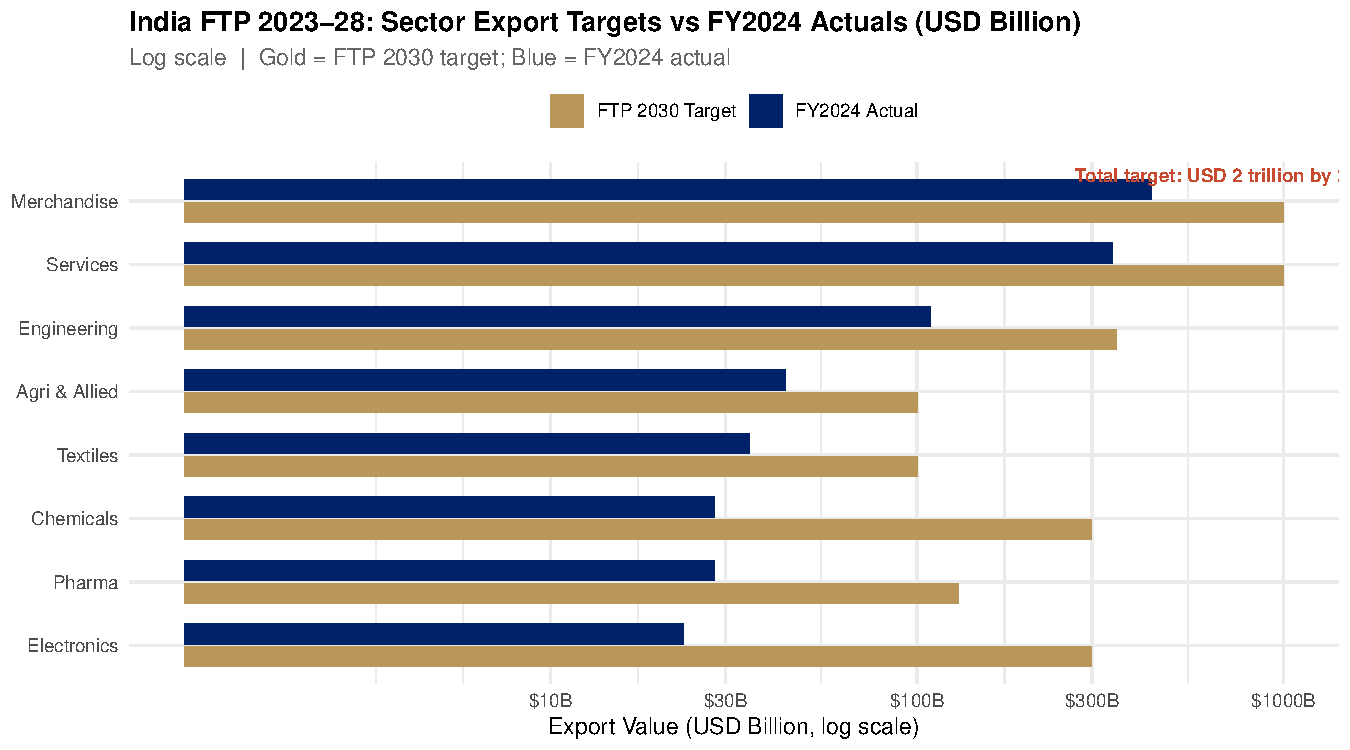
\includegraphics[keepaspectratio]{Lecture18_India_Agri_Trade_Policy_files/figure-beamer/fig-ftp-targets-1.pdf}}

}

\caption{\label{fig-ftp-targets}India's FTP 2023-28 targets USD 2
trillion in total exports by 2030. Agri and Allied targets USD 100B,
more than doubling the FY2024 actual of USD 43.7B. Log scale used for
wide value range. Source: DGFT, Foreign Trade Policy 2023-28.}

\end{figure}%
\end{block}
\end{frame}

\begin{frame}
\begin{block}{MEIS vs RoDTEP: India's Export Incentive Schemes}
\phantomsection\label{meis-vs-rodtep-indias-export-incentive-schemes}
\begin{figure}

\centering{

\pandocbounded{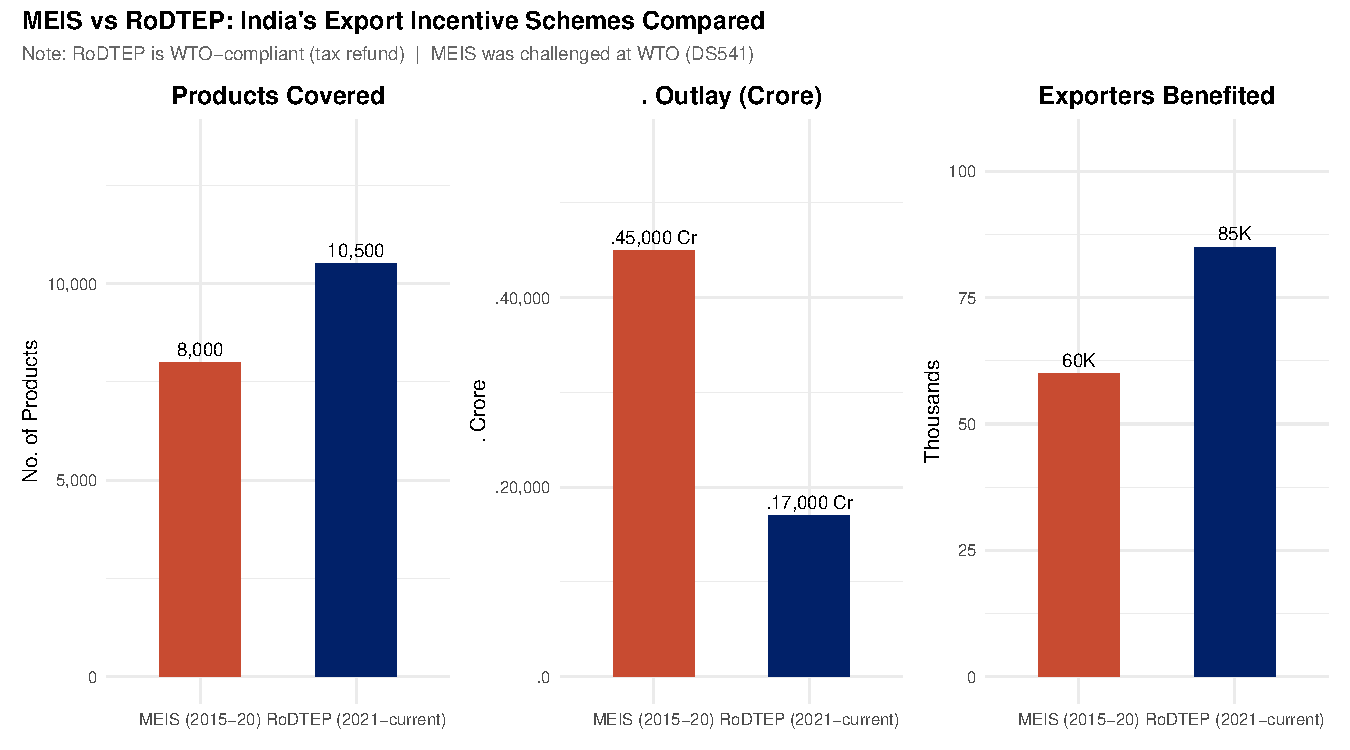
\includegraphics[keepaspectratio]{Lecture18_India_Agri_Trade_Policy_files/figure-beamer/fig-meis-rodtep-1.pdf}}

}

\caption{\label{fig-meis-rodtep}RoDTEP covers more products and
exporters than MEIS but at lower outlay, reflecting its design as a
WTO-compliant tax remission rather than a direct subsidy (MEIS was
challenged at WTO as DS541). Source: DGFT; WTO DS541 dispute record.}

\end{figure}%
\end{block}
\end{frame}

\begin{frame}
\begin{block}{Millets: why they matter for trade}
\phantomsection\label{millets-why-they-matter-for-trade}
\begin{itemize}
\tightlist
\item
  \textbf{2023 International Year of Millets} put ``Shri Anna'' on the
  global agenda
\item
  Nutrition demand: high fibre, gluten-free, ``health food'' positioning
\item
  Climate resilience: lower water needs than rice/wheat
\item
  India advantage: large producer base + varietal diversity
\item
  Export constraint: processing, packaging, certification, and
  consistent quality
\end{itemize}
\end{block}
\end{frame}

\begin{frame}
\begin{block}{India's millet portfolio (examples)}
\phantomsection\label{indias-millet-portfolio-examples}
\begin{itemize}
\tightlist
\item
  \textbf{Bajra (pearl millet):} Rajasthan, Gujarat, Haryana
\item
  \textbf{Jowar (sorghum):} Maharashtra, Karnataka
\item
  \textbf{Ragi (finger millet):} Karnataka, Andhra Pradesh
\item
  \textbf{Foxtail millet:} Telangana, Andhra Pradesh
\item
  \textbf{Kodo millet:} Madhya Pradesh, Chhattisgarh
\end{itemize}
\end{block}
\end{frame}

\begin{frame}
\begin{block}{APEDA and the millet export push}
\phantomsection\label{apeda-and-the-millet-export-push}
\begin{itemize}
\tightlist
\item
  Target: \textbf{\$100M} exports by FY2025 (from
  \textasciitilde{}\textbf{\$64M} in FY2023)
\item
  Market creation via global events and buyer outreach
\item
  Product formats: flour blends, snacks, pasta, RTE porridge
\item
  Winning requires: branding + lab testing + traceability
\item
  Market size: \textbf{\$11B by 2028} (health-food growth)
\end{itemize}

\note{Examples and diplomacy can be discussed orally (brands, G20
showcase) without crowding the slide.}
\end{block}
\end{frame}

\begin{frame}
\begin{block}{Geographical Indications as Trade Strategy}
\phantomsection\label{geographical-indications-as-trade-strategy}
\begin{columns}[T]
\begin{column}{0.55\linewidth}
\textbf{India's GI landscape (2024):}

\begin{itemize}
\tightlist
\item
  Total GIs registered: \textbf{400+}
\item
  Agricultural GIs: \textbf{230+} (largest category)
\item
  40 new GIs registered in FY2024
\end{itemize}

\textbf{Marquee agricultural GIs:}

\begin{longtable}[]{@{}lll@{}}
\toprule\noalign{}
Product & State & Price Premium \\
\midrule\noalign{}
\endhead
Darjeeling Tea & West Bengal & 40--60\% \\
Basmati Rice & Punjab/UP belt & 35--50\% \\
Alphonso Mango & Maharashtra (Ratnagiri) & 50--80\% \\
Malabar Black Pepper & Kerala & 25--35\% \\
Alleppey Green Cardamom & Kerala & 30--40\% \\
Guntur Sannam Chilli & Andhra Pradesh & 20--30\% \\
Coorg Arabica Coffee & Karnataka & 40--60\% \\
Kolhapuri Chilli & Maharashtra/Karnataka & 25--35\% \\
\bottomrule\noalign{}
\end{longtable}

A GI is, economically, a \textbf{geographic monopoly on a name.}
Producers in the designated region capture the premium; imitators cannot
legally use the name in protected jurisdictions.
\end{column}

\begin{column}{0.45\linewidth}
\textbf{The Basmati GI battle:}

India's application to protect ``Basmati'' as a GI at EU has been
contentious:

\begin{itemize}
\tightlist
\item
  \textbf{India's claim:} Only rice from designated districts of Punjab,
  Haryana, UP, Uttarakhand, J\&K qualifies
\item
  \textbf{Pakistan's objection:} Pakistani basmati (Super Kernel, Kainat
  varieties) has equal claim; both countries should be co-holders
\item
  \textbf{Stakes:} If EU grants India-only GI, Pakistan loses
  \textasciitilde\$1B annual EU basmati market access
\item
  \textbf{Decision pending 2024--25}
\end{itemize}

\textbf{Why GIs matter for development:}

Darjeeling tea's GI protection means the 87 estates and their workers
capture the ``Darjeeling'' brand premium --- which reaches £20--40 per
100g in UK specialty retail --- directly benefiting the 500,000+ workers
in those gardens.

GI policy is \textbf{distribution policy} --- it determines who captures
the value premium from cultural and geographic heritage.
\end{column}
\end{columns}
\end{block}
\end{frame}

\begin{frame}
\begin{block}{Challenges India Must Overcome}
\phantomsection\label{challenges-india-must-overcome}
\begin{columns}[T]
\begin{column}{0.5\linewidth}
\textbf{1. SPS compliance --- the entry ticket to premium markets:}

\begin{itemize}
\tightlist
\item
  EU rejections of Indian spices (EtO contamination, 2023): Everest and
  MDH spice brands recalled in Singapore, Hong Kong, USA; reputational
  damage to all Indian spice exporters
\item
  Aflatoxin in groundnuts, ochratoxin in coffee: recurring EU border
  rejections
\item
  FDA import alerts on Indian shrimp for antibiotic residues
\end{itemize}

\textbf{Required investment:} Farmer-level GAP training, village-level
residue testing, cold chain to reduce mycotoxin development.

\textbf{2. Value addition gap:}

India's agri export unit values are consistently below global averages
because we export raw and semi-processed commodities. Until the
processing sector scales, India will underperform its potential.

\textbf{3. Export restriction credibility:}

Rice bans (2023), wheat ban (2022), sugar quotas (2022), onion bans
(2023) --- India has a pattern of imposing sudden export restrictions to
manage domestic inflation. Each restriction: - Damages India's image as
a reliable supplier - Disrupts long-term trade relationships - Benefits
domestic consumers short-term but hurts farmers
\end{column}

\begin{column}{0.5\linewidth}
\textbf{4. Edible oil import dependence:}

\$14.2B annual import drag; NMEO-OP progress slow; structural
vulnerability to supply disruptions and price spikes.

\textbf{5. Cold chain and logistics:}

35M MT cold storage vs 90M MT requirement; 25--40\% post-harvest losses;
logistics cost 14\% of GDP vs 8\% in advanced economies.

\textbf{6. Market concentration:}

Rice at 28\% of agri exports; USA + UAE + Bangladesh = 32\% of
destinations. Shocks in any one product or market reverberate through
the whole system.

\textbf{The meta-challenge:}

India's domestic agricultural policy is designed primarily for
\textbf{food security and farmer welfare} --- these are legitimate and
important goals. But they frequently conflict with the objectives of
\textbf{export competitiveness and trade reliability.} Until India
develops better institutional mechanisms to reconcile these tensions,
export performance will remain hostage to domestic policy volatility.
\end{column}
\end{columns}
\end{block}
\end{frame}

\begin{frame}
\begin{block}{Opportunities for India's Agricultural Exports}
\phantomsection\label{opportunities-for-indias-agricultural-exports}
\begin{columns}[T]
\begin{column}{0.55\linewidth}
Despite the challenges, India faces an extraordinary window of
opportunity:

\textbf{1. Rising global food demand:}

World population reaches 10 billion by 2050; global food demand
projected to rise 50\% from 2012 levels. India's agricultural land,
labour, and knowledge base positions it as a key supplier.

\textbf{2. Indian diaspora --- the ready market:}

\textbf{\$4B+} in annual food imports by Indian diaspora communities
globally (USA, UK, Canada, Australia, Gulf). Indian diaspora is the most
rapidly growing food import segment in UK supermarkets (Tesco, Waitrose
Indian ranges up 35\% in 5 years). This is a market that \emph{wants}
Indian products and pays premiums.

\textbf{3. Organic and clean-label premium markets:}

Global organic food market: \$220B and growing 10\% annually. India has
4.5 million organic farmers --- the world's largest base --- but
captures only 0.5\% of global organic market. The upside potential is
immense.

\textbf{4. Millets and superfoods:}

First-mover advantage in a fast-growing \$11B global segment. India can
own the ``Shri Anna'' narrative globally.
\end{column}

\begin{column}{0.45\linewidth}
\textbf{5. FTA market access (India-UAE CEPA live; India-UK FTA
pending):}

Each FTA opens a new premium market without tariff headwinds. India-UAE
CEPA showed 28\% trade growth in year one.

\textbf{6. ASEAN's growing middle class:}

Southeast Asia's middle class (Indonesia, Vietnam, Philippines,
Thailand) is 400M+ and growing. Rising income = rising demand for
diverse, higher-quality foods including Indian spices, rice varieties,
processed snacks.

\textbf{7. Africa's rice gap:}

Sub-Saharan Africa imports \$7B in rice annually. India supplies 40\%.
With logistics investment (AIC --- Africa-India Connectivity), India can
deepen its dominant position in Africa's food import market.

\textbf{The opportunity is real.} But converting opportunity into
sustained export growth requires policy stability, infrastructure
investment, quality compliance, and institutional capacity. All of which
we have studied in this course.
\end{column}
\end{columns}
\end{block}
\end{frame}

\begin{frame}
\begin{block}{Core policy dilemma (1): MSP vs export competitiveness}
\phantomsection\label{core-policy-dilemma-1-msp-vs-export-competitiveness}
\begin{itemize}
\tightlist
\item
  Higher \textbf{MSP} raises farm incomes but can make exports
  uncompetitive
\item
  Example (wheat, 2023--24): MSP \textbf{₹2,275/quintal
  (\textasciitilde\$274/MT)} vs world price
  \textbf{\textasciitilde\$220/MT}
\item
  If exports still happen, it often requires \textbf{subsidies} or
  special channels
\item
  Political economy: farm support is sticky; export markets are
  price-sensitive
\item
  Result: policy must balance \textbf{income support} and \textbf{market
  access}
\end{itemize}
\end{block}
\end{frame}

\begin{frame}
\begin{block}{Core policy dilemma (2): food security vs export
reliability}
\phantomsection\label{core-policy-dilemma-2-food-security-vs-export-reliability}
\begin{itemize}
\tightlist
\item
  When domestic food prices rise, export bans/taxes protect consumers
\item
  But restrictions reduce farmers' export premium and incomes
\item
  Trade partners face supply shocks and search for alternative suppliers
\item
  Repeated bans weaken India's reputation as a reliable exporter
\item
  Long-run cost: lost market share even after restrictions end
\end{itemize}
\end{block}
\end{frame}

\begin{frame}
\begin{block}{Core policy dilemma (3): fiscal + WTO constraints}
\phantomsection\label{core-policy-dilemma-3-fiscal-wto-constraints}
\begin{itemize}
\tightlist
\item
  Food subsidy bill (FY2024): \textbf{₹2.05 lakh crore} (procurement +
  PDS + stocks)
\item
  Support shows up as WTO \textbf{domestic support (AMS / Amber Box)}
\item
  Compliance pressure increases as procurement expands
\item
  Reforms face strong political resistance
\item
  Bottom line: policy space is constrained by \textbf{budget + WTO
  rules}
\end{itemize}
\end{block}
\end{frame}

\begin{frame}
\begin{block}{Trade-offs cheat sheet}
\phantomsection\label{trade-offs-cheat-sheet}
\begin{itemize}
\tightlist
\item
  Farmer income → \textbf{high MSP} → fiscal cost + weaker export
  competitiveness
\item
  Consumer welfare → \textbf{export restrictions} → farmer loss +
  reputation damage
\item
  Export growth → \textbf{remove export taxes} → possible domestic price
  rise
\item
  WTO compliance → \textbf{reduce AMS} → farmer lobby resistance
\item
  Food security → \textbf{import restrictions} → higher domestic prices
\end{itemize}
\end{block}
\end{frame}

\begin{frame}
\begin{block}{Key insight from Econ 2203}
\phantomsection\label{key-insight-from-econ-2203}
Trade policy in agriculture distributes gains and losses among
\textbf{farmers, consumers, traders, and government}.

Economics helps by making these trade-offs explicit before we choose.
\end{block}
\end{frame}

\begin{frame}{Course Synthesis}
\phantomsection\label{course-synthesis}
\textbf{What Eighteen Weeks Has Taught Us}

\emph{Revisiting each major module through the lens of India's
agricultural trade reality}
\end{frame}

\begin{frame}
\begin{block}{Course synthesis (1): Theory → policy → BoP}
\phantomsection\label{course-synthesis-1-theory-policy-bop}
\begin{itemize}
\tightlist
\item
  \textbf{Trade theory (L1--L6):} comparative advantage shapes India's
  export basket
\item
  \textbf{Trade policy (L7--L8):} tariffs + incentives + MSP determine
  who gains/loses
\item
  \textbf{BoP constraint (L9--L10):} agri exports earn forex that
  finances key imports
\item
  Unifying idea: outcomes depend on \textbf{incentives + constraints}
\item
  India lens: agriculture is both a livelihood sector and a
  forex-earning sector
\end{itemize}
\end{block}
\end{frame}

\begin{frame}
\begin{block}{Course synthesis (2): Forex → WTO/AoA → SPS}
\phantomsection\label{course-synthesis-2-forex-wtoaoa-sps}
\begin{itemize}
\tightlist
\item
  \textbf{Forex (L11--L12):} INR moves change export realisation and
  import costs
\item
  \textbf{WTO/AoA (L13--L14):} rules constrain support but provide
  flexibilities (S\&DT)
\item
  \textbf{SPS (L15):} compliance is the entry ticket to premium markets
\item
  Unifying idea: \textbf{market access} increasingly depends on
  standards and credibility
\item
  India lens: coalitions (G-33/G-20) protect policy space in agriculture
\end{itemize}
\end{block}
\end{frame}

\begin{frame}
\begin{block}{Course synthesis (3): Institutions + procedures}
\phantomsection\label{course-synthesis-3-institutions-procedures}
\begin{itemize}
\tightlist
\item
  \textbf{Institutions (L16--L17):} APEDA/MPEDA/Boards/EIC
  operationalise exports
\item
  \textbf{Documentation:} contracts + certificates + customs make trade
  executable
\item
  \textbf{Quality infrastructure:} labs, traceability, cold chain reduce
  rejection risk
\item
  Policy without implementation fails
\item
  Implementation without credibility fails
\end{itemize}
\end{block}
\end{frame}

\begin{frame}
\begin{block}{Export vision 2030: target and what it implies}
\phantomsection\label{export-vision-2030-target-and-what-it-implies}
\begin{itemize}
\tightlist
\item
  Target: \textbf{\$100B} agri + food exports by 2030
\item
  Baseline: \textbf{\$43.7B} (FY2024)
\item
  Implied growth: \textbf{\textasciitilde12.5\% CAGR} (stretch)
\item
  Realistic waypoint: \textbf{\textasciitilde\$70B} with the right
  policies
\item
  Success needs quality investment + credibility (avoid repeated export
  bans)
\end{itemize}
\end{block}
\end{frame}

\begin{frame}
\begin{block}{Pillars for growth (I)}
\phantomsection\label{pillars-for-growth-i}
\begin{itemize}
\tightlist
\item
  Diversify beyond rice (processed food, fruits/veg, organic, millets)
\item
  New markets + FTAs (Africa, ASEAN, UK/EU access)
\item
  Quality investment (cold chain, labs, GAP training)
\item
  Value addition (RTE/processed/functionals)
\item
  GI + branding to earn price premia
\end{itemize}
\end{block}
\end{frame}

\begin{frame}
\begin{block}{Pillars for growth (II)}
\phantomsection\label{pillars-for-growth-ii}
\begin{itemize}
\tightlist
\item
  Reduce edible oil import dependence (saves forex)
\item
  Use WTO-compliant support (remission, not subsidies)
\item
  Strengthen SPS systems and traceability
\item
  Keep policy predictable (credibility = market share)
\item
  Coordinate public + private actors across the chain
\end{itemize}
\end{block}
\end{frame}

\begin{frame}
\begin{block}{Scenarios for FY2030}
\phantomsection\label{scenarios-for-fy2030}
\begin{itemize}
\tightlist
\item
  Conservative (5\% CAGR): \textbf{\$58B}
\item
  Base case (8\% CAGR): \textbf{\$69B}
\item
  Ambitious (12\% CAGR): \textbf{\$86B}
\item
  Stretch (\$100B): needs FTAs + processing clusters + no credibility
  shocks
\item
  Takeaway: the direction (higher value, diversified, compliant) is
  right
\end{itemize}
\end{block}
\end{frame}

\begin{frame}
\begin{block}{Final Thought: Agriculture and India's Development}
\phantomsection\label{final-thought-agriculture-and-indias-development}
\begin{columns}[T]
\begin{column}{0.6\linewidth}
India's agricultural trade is not merely an economic topic. It is the
story of \textbf{600 million lives.}

Every percentage point improvement in agricultural export earnings ---
whether from a better price for Darjeeling tea, or a new market for
Karnataka's tur dal, or an organic certification that enables Madhya
Pradesh soybean to command a premium in Hamburg --- translates into:

\begin{itemize}
\tightlist
\item
  \textbf{Higher farm incomes} for the cultivator who owns 1.08 hectares
  and whose children's education depends on the kharif season's outcome
\item
  \textbf{More rural employment} in post-harvest processing, cold chain
  logistics, packaging, and trade facilitation
\item
  \textbf{Better food security} through the forex earnings that fund
  India's critical imports and stabilise the current account
\item
  \textbf{National pride} --- in the Alphonso mango that Japanese
  consumers queue for, in the Coorg coffee that wins international
  awards, in the Indian ready-to-eat meal that a second-generation
  Indian in Leicester makes on a Tuesday night and calls it home
\end{itemize}

{This is why international trade policy in agriculture matters.}

And this is what Econ 2203 has been about.
\end{column}

\begin{column}{0.4\linewidth}
\textbf{A kilo of Kalaburagi tur dal travels from a Karnataka farmer to
a diaspora kitchen in Leicester.}

We began Lecture 16 with this image.

We can now trace every step:

\begin{itemize}
\tightlist
\item
  The IEC and RCMC that licensed the export
\item
  The FOB contract and LC that financed it
\item
  The Phytosanitary Certificate and Shipping Bill that cleared it
\item
  The APEDA-linked FPO that aggregated the smallholders
\item
  The RoDTEP scrip that rewarded the exporter
\item
  The comparative advantage that made it competitive
\item
  The WTO rule that kept the market open
\end{itemize}

\textbf{That journey is Econ 2203.}
\end{column}
\end{columns}
\end{block}
\end{frame}

\begin{frame}
\begin{block}{Key Takeaways for the Examination and for Life}
\phantomsection\label{key-takeaways-for-the-examination-and-for-life}
\textbf{Five messages to carry beyond this classroom:}

\begin{enumerate}
\item
  \textbf{{Comparative advantage, not absolute advantage, drives
  specialisation}} --- India need not be the cheapest in everything; it
  only needs a relative cost advantage in what it exports. This is
  Ricardo's enduring insight.
\item
  \textbf{{Free trade maximises efficiency, but food security requires
  nuanced policy}} --- the tension between these goals is real,
  legitimate, and never fully resolved. The best economists acknowledge
  the trade-offs rather than pretending they do not exist.
\item
  \textbf{{WTO rules constrain AND protect India's agricultural policy
  space}} --- India must simultaneously defend its right to support
  farmers and work to ensure global rules are fair for developing
  country agriculture. Both are valid positions.
\item
  \textbf{{SPS compliance is the critical bottleneck for India's agri
  export growth}} --- not tariffs, not logistics, not finance. The
  moment India's spice, seafood, or fresh produce consistently meets the
  safety standards of the EU, USA, and Japan, billions of dollars of
  additional export value become accessible.
\item
  \textbf{{Value addition, not raw commodity exports, is the path to
  \$100 billion}} --- India must move from exporting raw cashew to
  exporting cashew butter; from raw turmeric to curcumin capsules; from
  frozen shrimp to ready-to-cook seafood meals. That transition is the
  work of the next decade.
\end{enumerate}
\end{block}
\end{frame}

\begin{frame}
\begin{block}{Examination Information}
\phantomsection\label{examination-information}
\begin{columns}[T]
\begin{column}{0.55\linewidth}
\textbf{Final Examination --- Econ 2203:}

\textbf{Format:}

\begin{itemize}
\tightlist
\item
  Part A: 20 short-answer questions (2 marks each) --- 40 marks
\item
  Part B: 4 essay questions from 6 choices (15 marks each) --- 60 marks
\item
  Total: 100 marks; Duration: 3 hours
\end{itemize}

\textbf{Emphasis areas (all lectures equally weighted):}

\begin{itemize}
\tightlist
\item
  Trade theory: comparative advantage, HO theorem, ToT
\item
  Tariffs, quotas, ERP calculations, optimal tariff
\item
  WTO Agreement on Agriculture: three pillars, amber/green/blue boxes
\item
  SPS Agreement: MRL, risk assessment, India's challenges
\item
  Balance of Payments and forex: current account, J-curve
\item
  India's trade policy: FTP 2023--28, RoDTEP, APEDA, MPEDA
\item
  Export procedures: IEC, Shipping Bill, LC, key documents
\end{itemize}

\textbf{Numerical questions:}

Be prepared to calculate: ERP, welfare effects of tariff (DWL), terms of
trade, exchange rate pass-through.
\end{column}

\begin{column}{0.45\linewidth}
\textbf{Suggested revision strategy:}

\textbf{Week 1 before exam:} - Re-read lecture slides for all 18
lectures - Focus on definitions and institutional names (APEDA, ICEGATE,
RoDTEP, NRCP) - Practise the tariff welfare diagram from memory

\textbf{Week 2 before exam:} - Attempt 2015--2024 past paper questions -
Practise numerical problems on ERP, ToT, DWL - Revise India-specific
data: FY2024 export value, top products, WTO bound rates

\textbf{A final word from your instructor:}

You have worked hard across 18 weeks on a subject that matters --- not
just for your examination, but for understanding one of the most
consequential policy domains in India's development journey.

\textbf{Thank you. Good luck. Go well.}
\end{column}
\end{columns}
\end{block}
\end{frame}

\begin{frame}{Appendix}
\phantomsection\label{appendix}
\begin{block}{Additional Resources}
\phantomsection\label{additional-resources}
\begin{columns}[T]
\begin{column}{0.5\linewidth}
\textbf{Further Reading}

\begin{itemize}
\tightlist
\item
  Lecture notes and APEDA/WTO official documents
\item
  APEDA Annual Report 2023-24
\item
  RBI/DGCI\&S/APEDA databases for latest data
\end{itemize}
\end{column}

\begin{column}{0.5\linewidth}
\textbf{Key Data Sources}

\begin{itemize}
\tightlist
\item
  DGCI\&S: India's merchandise trade
\item
  RBI: Balance of payments data\\
\item
  APEDA: Agricultural export statistics
\item
  WTO: Tariff and trade databases
\end{itemize}
\end{column}
\end{columns}
\end{block}
\end{frame}




\end{document}
